%!TEX root = these.tex

\begin{appendices}
% \appendixpage
\clearpage
\let\clearpage\relax
\vspace*{\fill}
\begin{center}
  \Huge\bfseries Annexe
\end{center}

\vspace*{\fill}
% \noappendicestocpagenum
% \addappheadtotoc
\chapter{Annexe}
\label{appendix:annexe}
\section{Annotations de vidéos, données complémentaires}

	\begin{figure}[!htb]
		\begin{subfigure}[t]{\subImgWclicks}
			\centering
			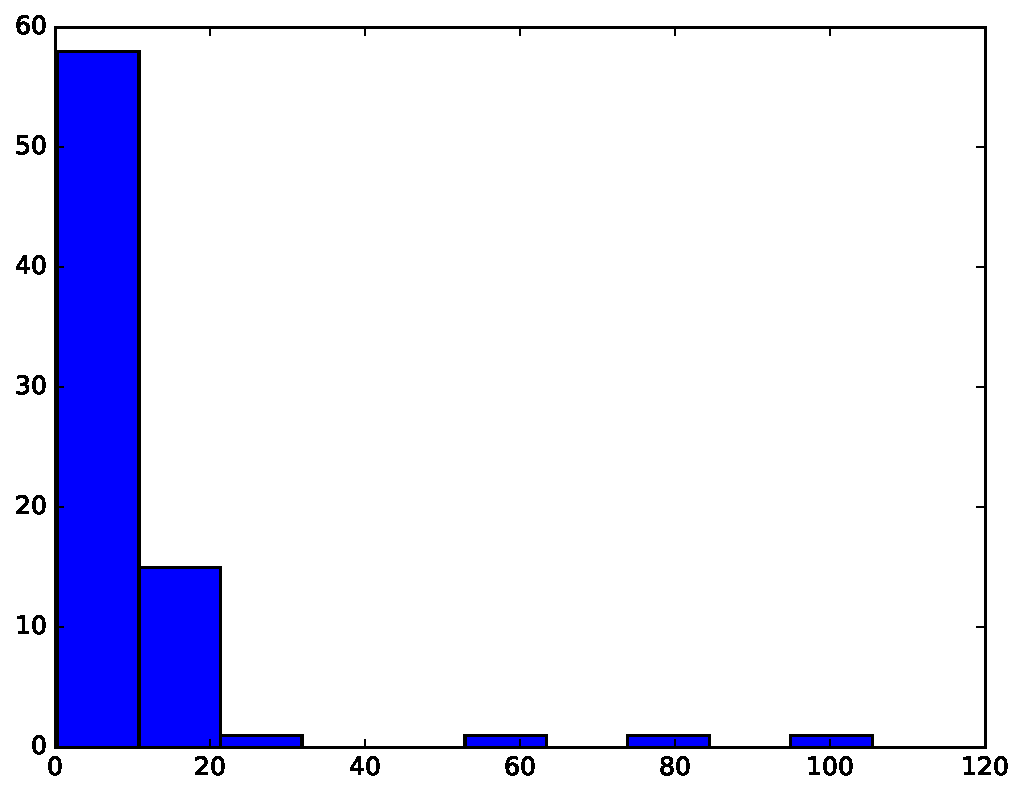
\includegraphics[width=\textwidth]{figures/annexe/bulletA_filteredSpeed}
			\caption{Vitesses.}
			\label{fig:bulletA_filteredSpeed}
		\end{subfigure}
		~
		\begin{subfigure}[t]{\subImgWclicks}
			\centering
			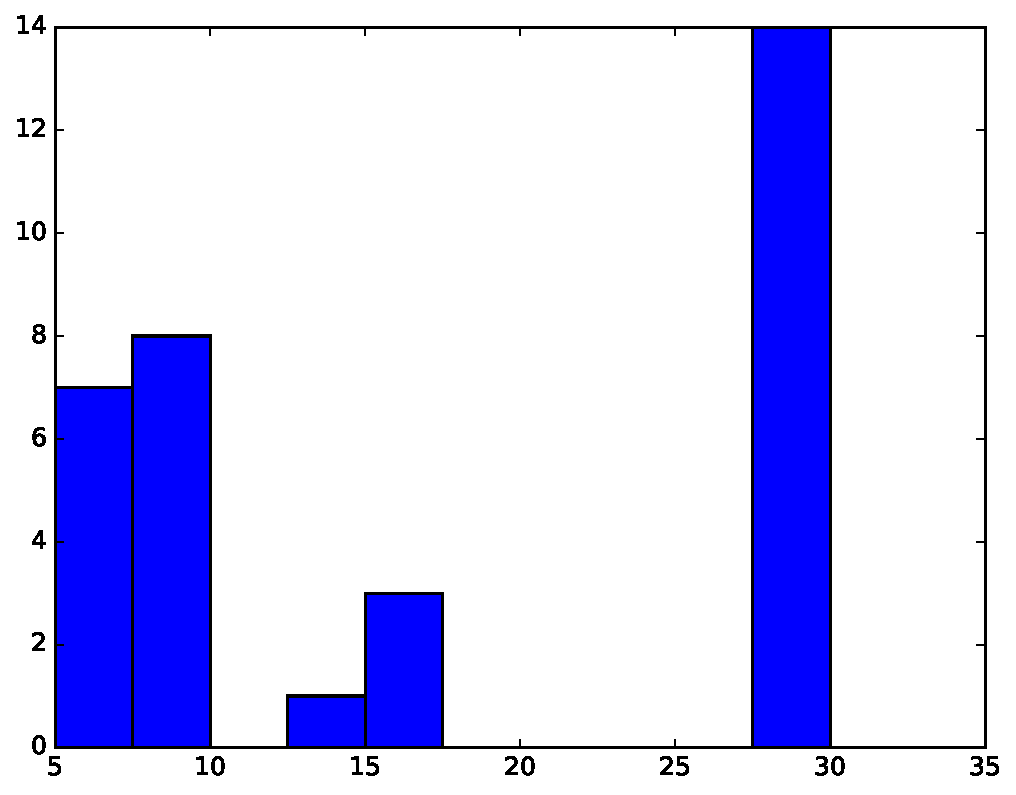
\includegraphics[width=\textwidth]{figures/annexe/bulletA_frequency}
			\caption{Fréquences.}
			\label{fig:bulletA_frequency}
		\end{subfigure}
		~
		\begin{subfigure}[t]{\subImgWclicks}
			\centering
			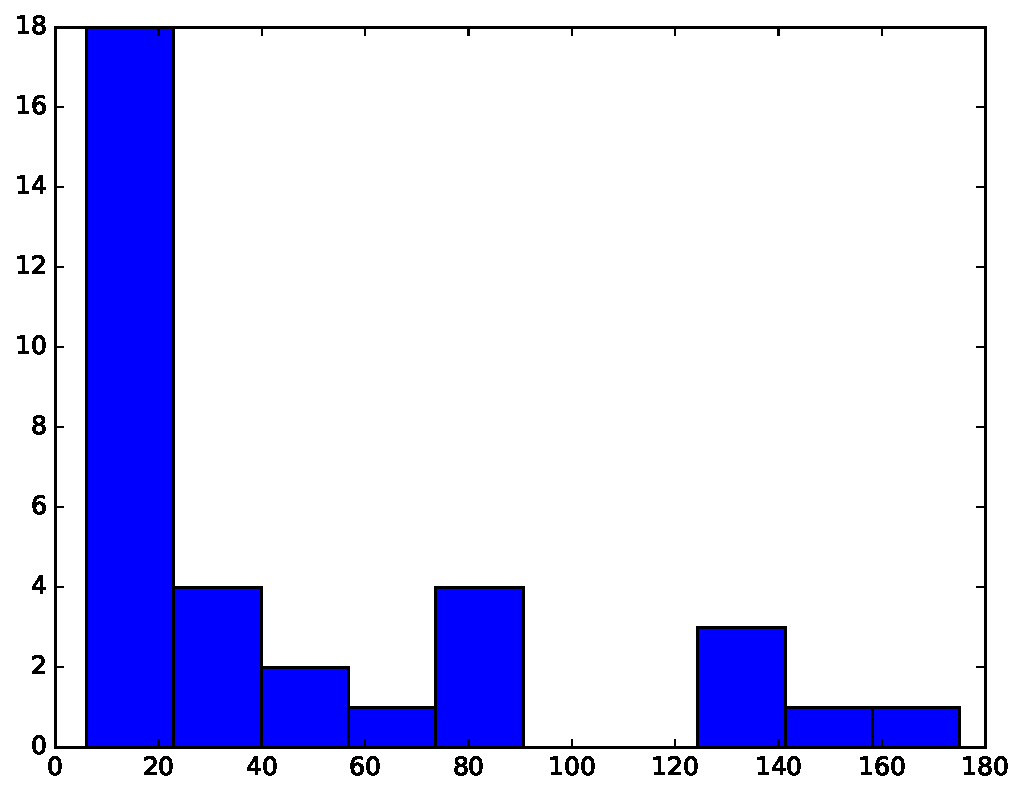
\includegraphics[width=\textwidth]{figures/annexe/bulletA_angle}
			\caption{Angles.}
			\label{fig:bulletA_angle}
		\end{subfigure}
		\caption[Histogrammes pour la balle de pistolet]{Histogrammes pour la balle de pistolet.}
		\label{fig:histBullet}
	\end{figure}
	
\begin{table}
	\centering
	\begin{tabular}{c c c c c c c c c}
		$V_{max}$	& $\overline{V}$	& $\sigma_{V}$	& $F_{max}$	& $\overline{F}$	& $\sigma_{F}$	& $A_{max}$	& $\overline{A}$	& $\sigma_{A}$	\bigstrut[b] \\ \hline

		105,45		& 10,27				& 15,96			& 30,00		& 18,24				& 10,41			& 175,06	& 45,23				& 47,83			\bigstrut[t] \\
	\end{tabular}
	\caption[Statistiques pour la vidéo de balle de pistolet]{Statistiques pour la vidéo de balle de pistolet.}
	\label{tab:bulletA_stats}
\end{table}



%\chapter{Annexe B}
%\label{appendix:annexeB}




\end{appendices}